\ProvidesFile{ch2.tex}[Chapter2]

\chapter{Bromodomain protein 4 and chromatin organization}
\ix{physics//Physics appendix}

The interplay between chromatin structure and phase-separating proteins is an emerging topic in cell biology with implications for understanding disease states. Here, we investigate the functional relationship between bromodomain protein 4 (BRD4) and chromatin architecture. By combining molecular dynamics simulations with live-cell imaging, we demonstrate that BRD4, when phosphorylated at specific N-terminus sites, significantly impacts nucleosome nanodomain (NN) organization and dynamics. Our findings reveal that enhanced chromatin binding activity of BRD4 condenses NNs, while both loss or gain of BRD4 chromatin binding reduced diffusion of single nucleosomes, suggesting a role for BRD4 in the regulation of nanoscale chromatin architecture and the chromatin microenvironment. These observations shed light on the nuanced regulation of chromatin structure by BRD4, offering insights into its role in maintaining the nuclear architecture and transcriptional activity.

\section{Introduction}

The cell nucleus is a densely packed environment with chromatin comprising a dominant component. The compartmentalization of chromatin with other intranuclear components by phase separation is therefore an efficient strategy to ensure precise spatial and temporal coordination of complex dynamics. A growing number of phase separated nuclear bodies have been identified, including transcriptional condensates1,2, nuclear speckles3, and DNA damage repair foci4; however, the interplay of phase separated condensates with the underlying chromatin structure remains poorly understood. Transcriptional condensates have been identified as an ideal model to study the kinetic and thermodynamic contributions of chromatin substrate binding, as the ability of transcriptional activators to both condense and bind chromatin is well established1,5–8. Here, we extend this effort by investigating the regulation of chromatin structure by phase separated transcriptional condensates. We focus on the BRD4 protein - a well-studied transcriptional activator that localizes to acetylated chromatin sites9, recruits pTEF-b10, and initiates transcription of key genes involved in signal response, immunity, and oncogenesis10.
	The BRD4 long isoform is characterized by structured N-terminal tandem acetyl-lysine binding bromodomains and an extra-terminal domain, connected by intrinsically disordered regions11. Perhaps the most fundamental of BRD4 functions is the ability to bind to acetylated chromatin through bromodomain 1 (BD1) and bromodomain 2 (BD2) that are in tandem within the N-terminal part of the protein. BRD4 inhibitors such as (+)-JQ1 competitively bind to the acetyl-binding pocket of BRD4, displacing BRD4 from chromatin12. It is also well known that BRD4 association with acetylated chromatin is enhanced by casein kinase II (CK2)-mediated phosphorylation of seven N-terminus phosphorylation sites (NPS), followed by intramolecular rearrangement13 of BRD4 protein and/or BRD4 dimerization13,14.
	Recent studies have demonstrated that BRD4 is present in discrete nuclear bodies that occur at super-enhancers, which exhibit properties of other well-studied biomolecular condensates, including rapid recovery of fluorescence after photobleaching and sensitivity to 1,6-hexanediol, which disrupts liquid-like condensates (Sabari 2018). Both BRD4 long and short isoform are found in phase separated condensates in the nucleus and are associated with active gene transcription1. Importantly, CK2-mediated NPS phosphorylation state regulates chromatin binding activity of BRD413 as well as BRD4 phase separation11. This has led to the conclusion that phosphorylation of BRD4 inhibits interaction with chromatin and reduces phase separation, while remaining necessary for active gene transcription. Moreover, phosphorylated and unphosphorylated BRD4 form different molecular associations – transient polyvalent associations of unphosphorylated BRD4 contrast with the stable dimeric interaction and chromatin binding of phosphorylated BRD414. We therefore speculated that BRD4 chromatin binding may be necessary for maintaining NN structure and single nucleosome dynamics. 

\section{Results}

\subsection{Colocalization of BRD4 mutants with nucleosome nanodomains}

	To address the role of BRD4 binding and phase separation on chromatin structure, we express FLAG-tagged BRD4 mutants with NPS or bromodomain mutations in HeLa cells and measure their effects on chromatin organization. In particular, we express a constitutively phosphorylated (7D mutant), constitutively unphosphorylated (7A mutant), and bromodomain-deactivated (BD mutant) protein (Figure 1a,b). Colocalization analysis of FLAG-tagged 7A/7D BRD4 mutants with NNs using nearest neighbor distance distribution function G(r) showed an obvious colocalization of these mutants with NNs with respect to complete spatial randomness. 

\begin{figure}[t]
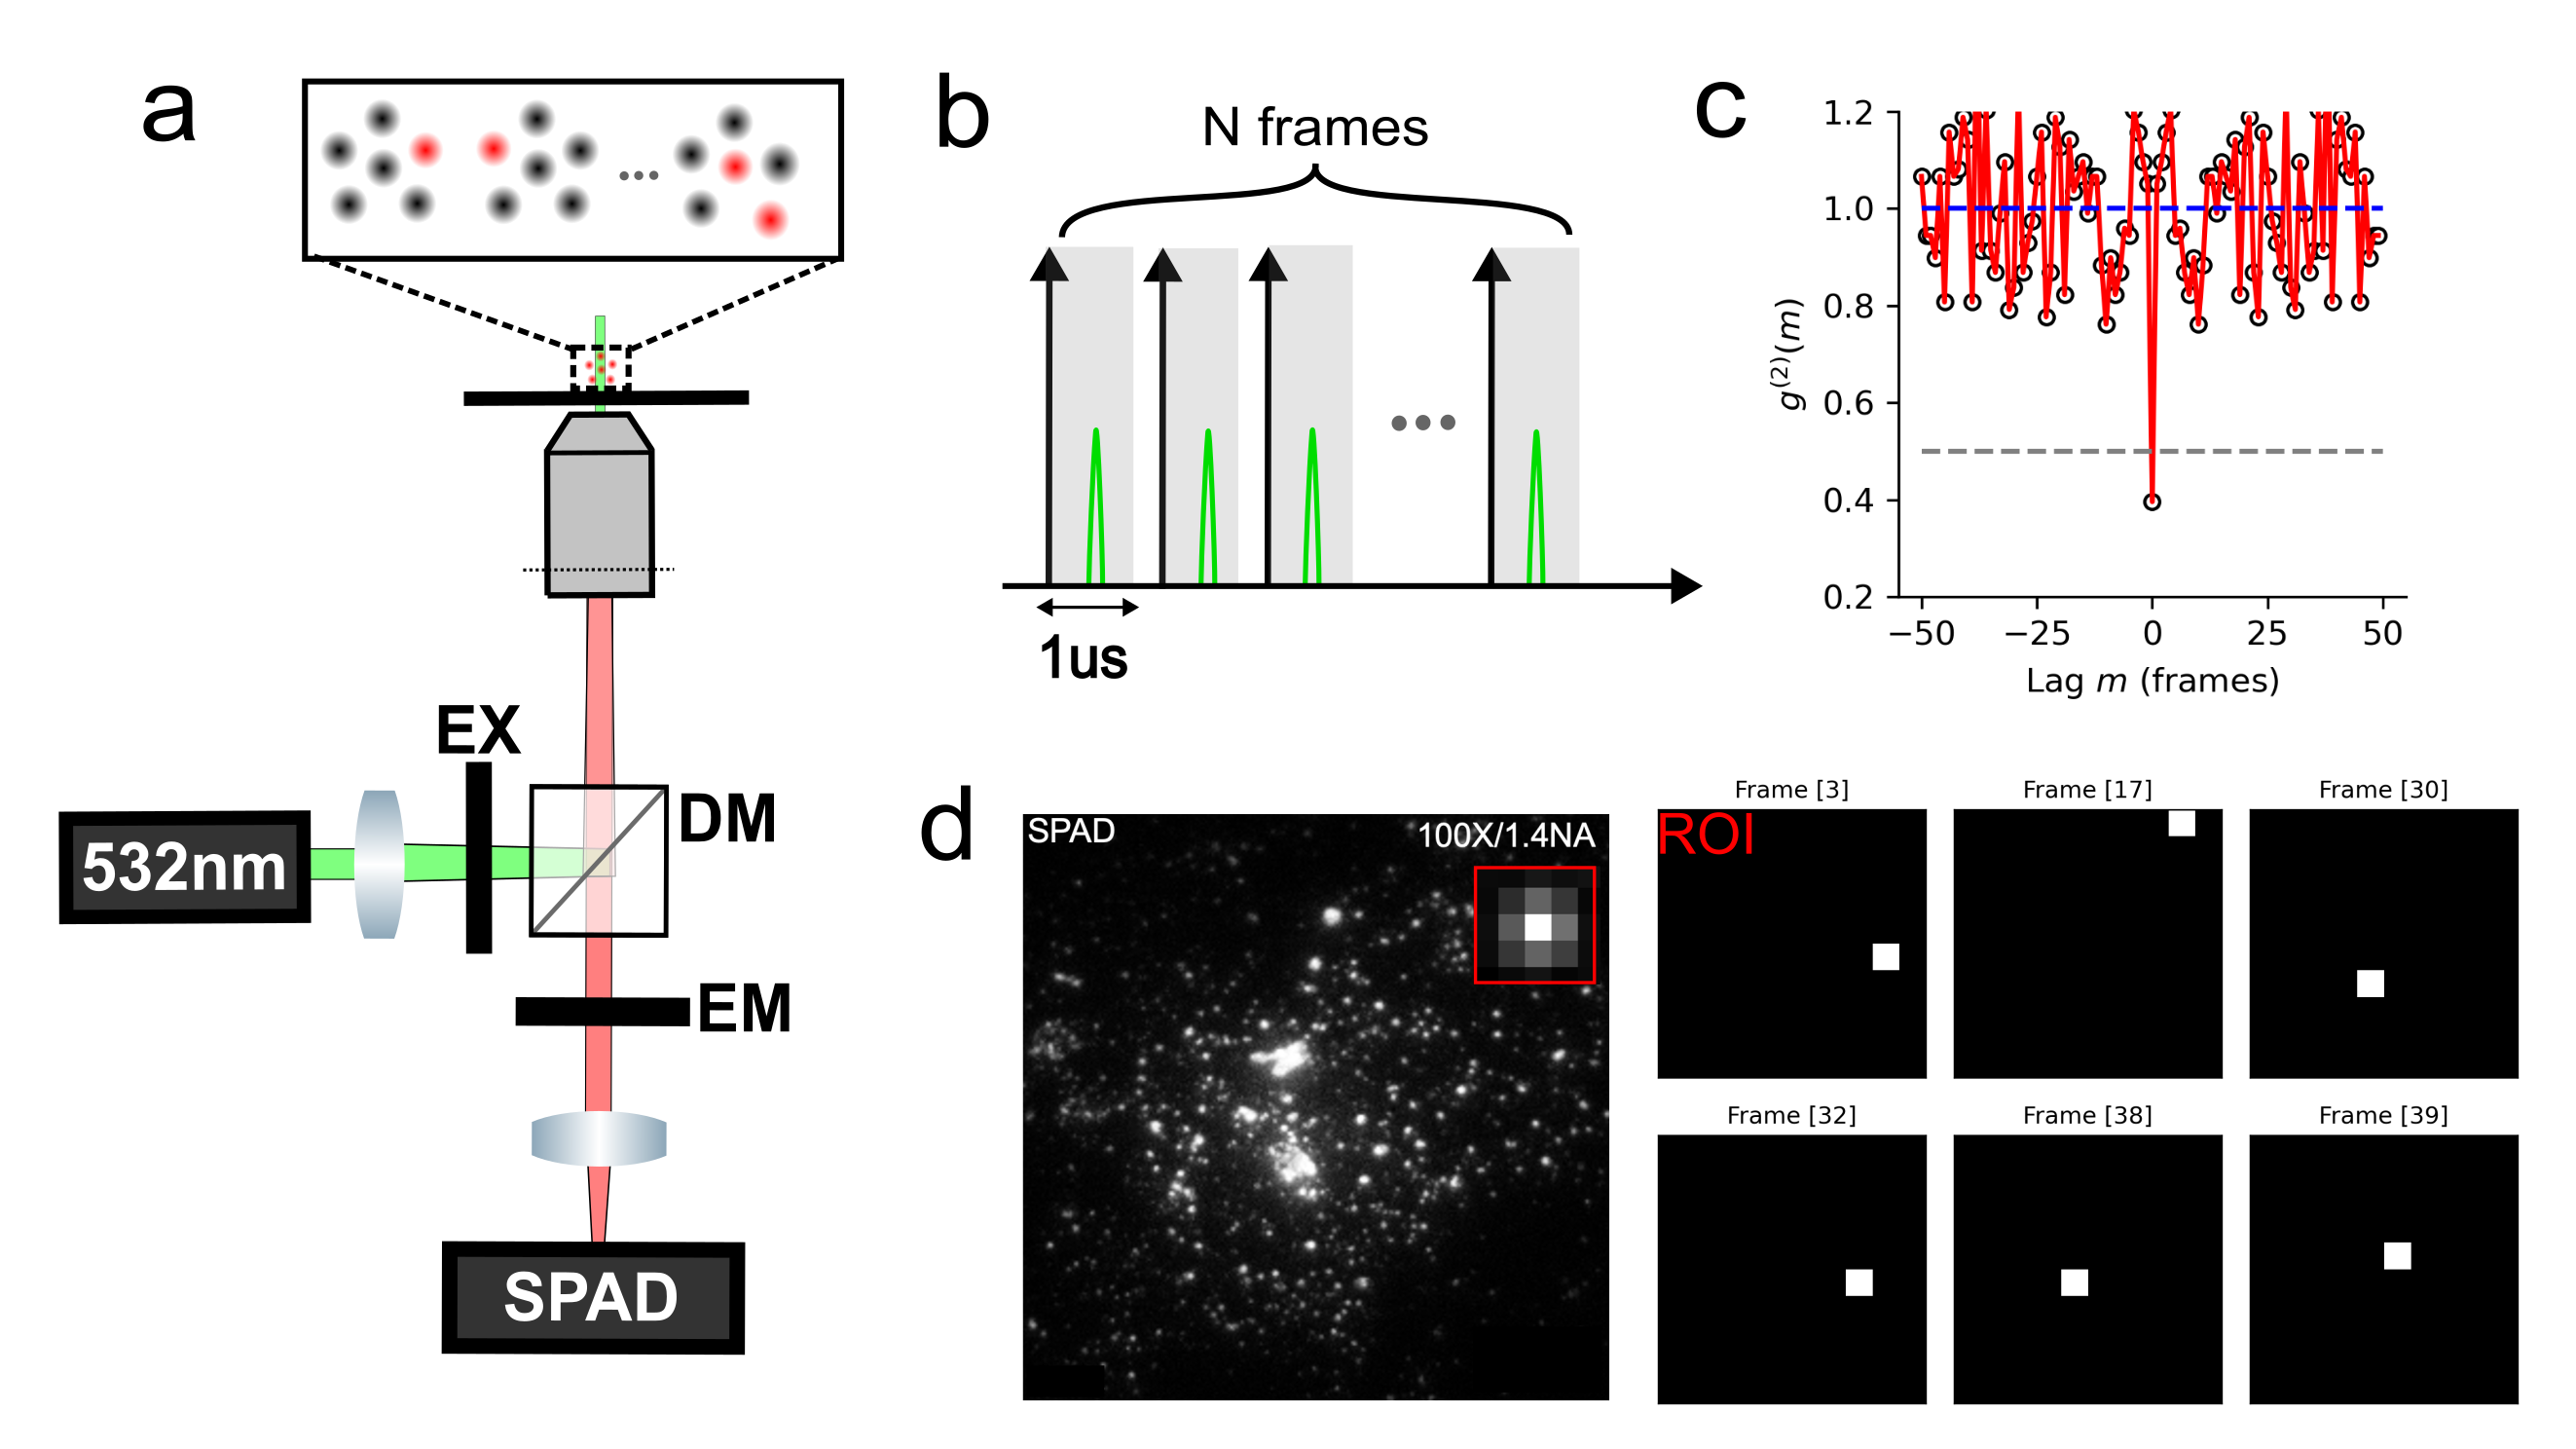
\includegraphics[width=\textwidth]{/Users/cwseitz/git/cwseitz.github.io/docs/phd/brd4/brd4/media/Figure-0.png}
\caption{}
\end{figure}
	
\subsection{Chromatin structure and dynamics}

To assess the functional role of BRD4 in maintaining the NN environment, we interrogated the dynamics of NNs, as well as their structure, in the presence of BRD4 mutants. Histone H2B was tagged with HaloTag15 (H2B-Halo), to which a fluorescent ligand JaneliaFluor646 (JF646) can bind specifically in a living cell. Low concentrations of JF646 were used to obtain sparse labeling of nucleosomes for single-nucleosome imaging (Figure 2a,b). JF646-labeled nucleosomes in Hela cells were recorded at 10fps (∼200 frames, 20 s total) and a reduced diffusion coefficient was measured in cells expressing 7A, 7D, and BD mutants, with respect to cells expressing the wild-type BRD4 protein (Figure 2c,d). We then conducted super resolution imaging of nucleosome nanodomains using direct stochastic optical reconstruction microscopy (dSTORM) by promoting JF646 fluorescence intermittency with a cysteamine buffer (Figure 3a,c). JF646 is known to exhibit a transient fluorescent state lasting tens to hundreds of milliseconds and stable dark state lasting hundreds of milliseconds to seconds16. Two color imaging of H2B-Halo-JF646 and GFP-tagged BRD4 shows that BRD4 and NNs form complementary biomolecular condensates in the nucleus, consistent with current models of BRD4 chromatin reading mechanism (Figure 3b). Ensemble averages of Besag’s L-function showed an increase in NN compaction in cells expressing the 7D BRD4 mutants, while all other groups were consistently indistinguishable from WT cells (Figure 3d).  

\begin{figure}[t]
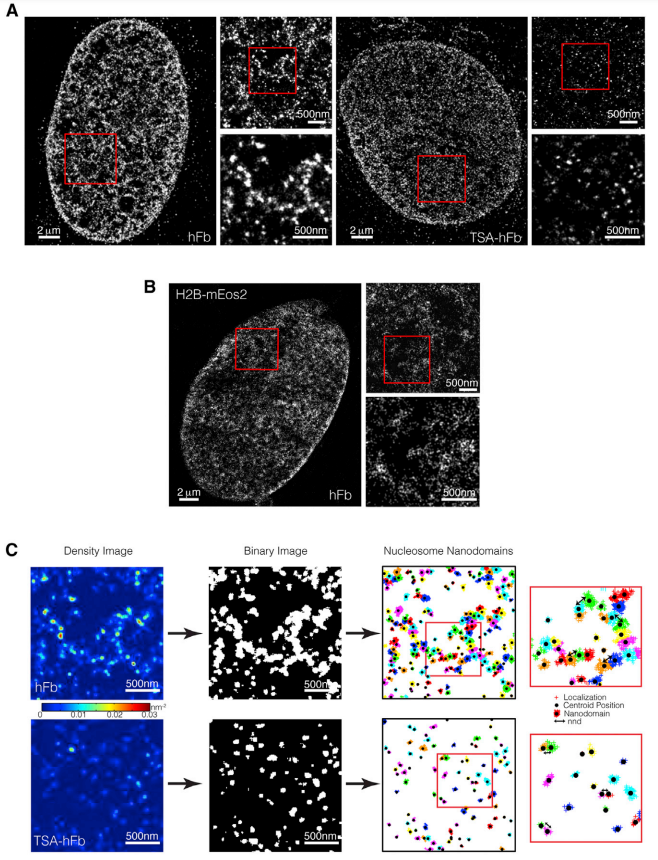
\includegraphics[width=\textwidth]{/Users/cwseitz/git/cwseitz.github.io/docs/phd/brd4/brd4/media/Figure-1.png}
\caption{}
\end{figure}

\begin{figure}[t]
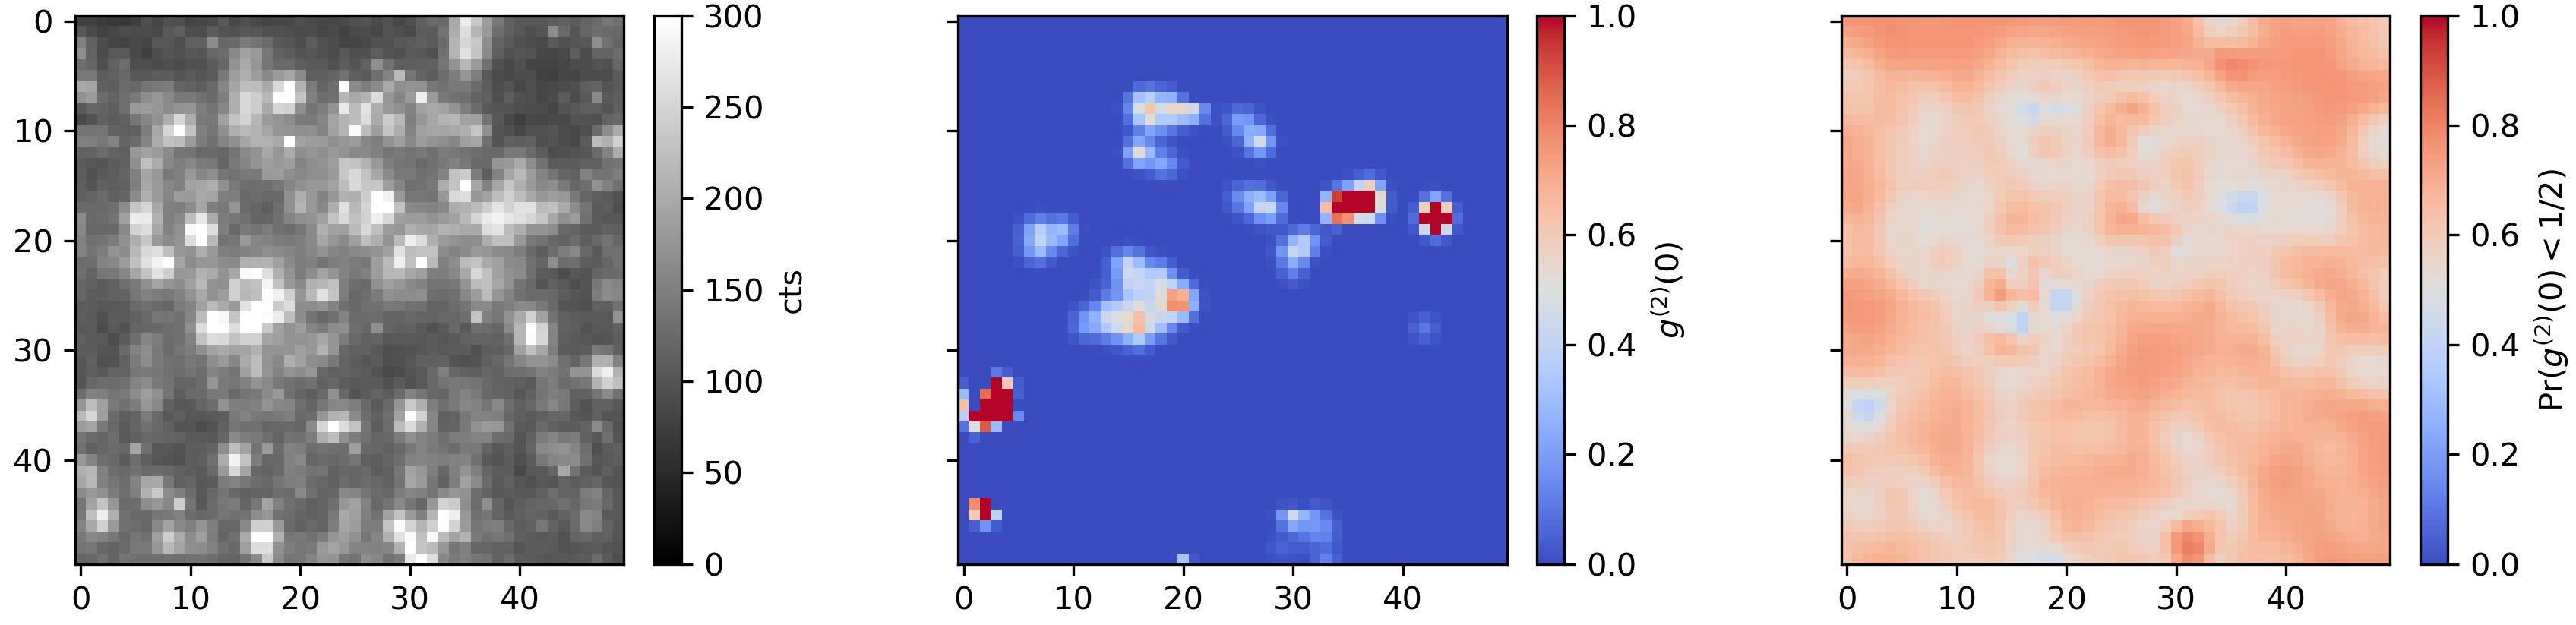
\includegraphics[width=\textwidth]{/Users/cwseitz/git/cwseitz.github.io/docs/phd/brd4/brd4/media/Figure-2.png}
\caption{}
\end{figure}

\subsection{Heteropolymer model}

To interpret our experimental findings, we adopt a heteropolymer chromatin model to capture the interaction of chromatin with multivalent BRD4-like binders (Figure 4a). The heteropolymer consists of a coarse-grained bead-and-spring chain composed of $N_b=200$ beads, connected by harmonic bonds with equilibrium length $r_0$ whose energy is defined as

\begin{equation*}
U_{AB}(r_{ij})=\frac{\kappa}{2}(\lvert r_{ij}\lvert-r_0)^2
\end{equation*}

where $r_{ij}$ is a vector connecting the center of a bead of type $i$ to a bead of type $j$ and $i,j \in (A,B)$. In all simulations, we assume $\kappa=90k_{B}T{r_0}^2$ where $k_{B}$ is Boltzmann’s constant and $r_0=200$nm. Random beads in the chain are selected to represent locally unacetylated (A-type particles) and acetylated chromatin (B-type particles).  B-type particles undergo multivalent interactions with a third group of C-type particles, which can promote cross-linking of the polymer. We presume a Bernoulli probably of $p=0.3$ for any given bead to be in an acetylated-like state. Interaction of multivalent chromatin binders with chromatin beads are then mediated by the following potential:

\begin{equation*}
U_{BC}\left(r_{ij}\right)=\epsilon\left(1-\left(\frac{\lvert r_{ij}\lvert}{R_0}\right)^2\right)^3
\end{equation*}

where $R_0=200$nm. The potential $U_{BC}$ is considered over a domain $0\leq\lvert r_{ij}\lvert\leq 2 R_0$ In all simulations, ten replicates were run for each condition tested. A and B type particles within the chromatin polymer have repulsive interactions with $\epsilon = +10k_{B}T$. Binding energy of the acetylated beads with binders was varied with $\epsilon_{I} = 0 k_{B}T,\epsilon_{II} = -20k_{B}T,\epsilon{III}=-40k_{B}T$ (Figure 4b). The dynamics of chromatin chains are approximated by Brownian dynamics within a cubic box with side length of 10um and periodic boundary conditions. Brownian dynamics follows the stochastic differential equation.

\begin{figure}[t]
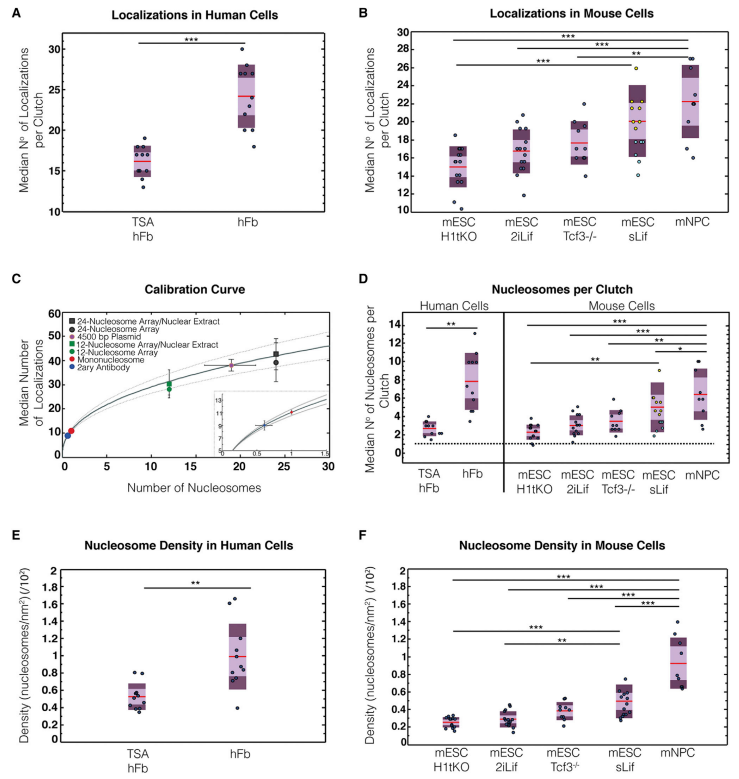
\includegraphics[width=\textwidth]{/Users/cwseitz/git/cwseitz.github.io/docs/phd/brd4/brd4/media/Figure-3.png}
\caption{}
\end{figure}

\begin{equation*}
\dot{\bold{r}} = \gamma^{-1}\nabla U(\bold{r}) +\sqrt{2 k_{B}T}\gamma^{-1/2}\xi(t)
\end{equation*}

where $\gamma$ is a diagonal friction tensor and $\xi(t)$ is a three-dimensional delta-correlated white noise $\langle \xi(t)\xi(t+\tau)  = \delta(t,t+\tau)$. Integrating the Brownian dynamics showed an overall reduction of the variance of the diffusion coefficient $D$ of single beads, and linear scaling of the diffusion coefficient with respect to temperature (Figure 4e).

\section{Discussion}

Our data support the model that phosphorylated and unphosphorylated BRD4 form different molecular associations in the nucleus. BRD4 nuclear localization is only weakly affected by bromodomain inhibition with monovalent BET inhibitors, while exposure to phase separation inhibitors such as 1,6 Hexanediol have a significant effect on BRD4 localization in the nucleus11. Therefore, nascent BRD4 condensates are likely seeded by unphosphorylated BRD4, followed by CK2-mediated phosphorylation, promoting chromatin interactions mediated by phosphorylated form. The stable dimeric interaction and binding of phosphorylated BRD4 to acetylated chromatin would then mediate control of the chromatin architecture by promoting cross-linking of the chromatin fiber and acting a molecular ‘bridge’ between transcriptional condensates with chromatin. Concurrently, reduced diffusivity of single nucleosomes with no overall change in NN compaction (cross-linking) in the unphosphorylated mutant is a natural result of molecular crowding resulting from overexpression of a constitutively phase separating protein, capable of multivalent interactions. 

\section{Materials and Methods}

\subsection{Cell lines, cell culture conditions, and transfection}

Hela cells were cultured in DMEM supplemented with 10 percent fetal bovine serum (Gibco) at 37C 5 percent CO2 in a humidified incubator. Cultures were tested routinely for mycoplasma contamination; all tests were negative. For super-resolution experiments, cells were seeded in a 35mm FluoroDish (WPI), and transiently transfected using Lipofectamine 3000 with pBREBACK-H2BHalo plasmid (Addgene plasmid 91564) (ThermoFisher), pcDNA5-Flag-BRD4-7A (Addgene Plasmid 90006), pcDNA5-Flag-BRD4-7D (Addgene Plasmid 90007), pCDNA5-Flag-BRD4-BD (Addgene Plasmid 90005), pcDNA5-Flag-BRD4-WT (Addgene Plasmid 90331)

\subsection{Super-resolution imaging of nucleosome nanodomains in living cells}

After transient transfection, H2B-Halotag Hela cells were incubated with 3pM JF646 HaloTag ligand overnight. Cells were imaged in a dSTORM photoswitching buffer containing 100mM MEA, 50 ug/ml Glucose Oxidase, and 3.4 mg/ml Catalase (Sigma). Buffer pH was adjusted to ~8 using HCl. Movies were collected using a custom Olympus IX83 microscope body equipped with an Olympus 60X 1.25NA oil-immersion objective. During imaging cells were maintained at 37C and 5 percent CO2 in a stage top incubator (Tokai Hit). Images were projected onto an ORCA-Fusion sCMOS camera (Hamamatsu) and 2000 frames were captured at 100fps. The microscope was controlled using Micromanager software. HaloTag-JF646 molecules were imaged using oblique illumination with a 640nm laser (Excelitas) held at 20mW, as measured at the back focal plane of the objective. Super resolution reconstructions were obtained using the ThunderSTORM ImageJ plugin. Background signal was subtracted using a rolling ball filter with radius of 10 pixels. Spots were fit using an integrated Gaussian point spread function model with maximum likelihood estimation17,18. Experimental conditions for single molecule tracking are nearly identical. However, H2B-Halotag Hela cells were incubated with 3pM JF646 HaloTag ligand. HaloTag-JF646 molecules were illuminated at 10mW, 100 frames were captured at 10fps. 

\begin{equation*}
K(r) =\frac{a}{n(n-1)}\sum_{ij}{I(d_{ij}\ \le r)}\;\;\; L(r)\ \sqrt{\frac{K(r)}{\pi}}
\end{equation*}

Precise x,y positions of the fluorophores are obtained, Besag’s L-function L(r) is used to analyze the clustering. The L-function is the following transformation of Ripley’s K-function K(r) 


where $a$ is the area of the window, $r$ is the distance between, $n$ is the number of data points and the sum is taken over all pairs of fit coordinates as shown in equation XXX. The indicator function is given by $I(d_{ij}\le r)$ and equals 1 if the distance is less than or equal to $r$. To measure degree of clustering, we use $L(r)-r$, which measures the deviation of a point pattern from complete spatial randomness (CSR). 

\subsection{Colocalization of BRD4 mutants with nucleosome nanodomains}

We colocalize FLAG-tagged 7A/7D BRD4 mutants with nucleosome nanodomains by simultaneous FLAG immunofluorescence with imaging of sparsely labeled of H2B-JF646. Puncta were detected in both channels using the Laplacian of Gaussian (LoG) detection algorithm to generate a multi-type point pattern. We then computed the nearest neighbor distance distribution function $G(r)$, which is the cumulative distribution function of the distance from a random H2B-JF646 puncta to the nearest BRD4-FLAG puncta. This function was computed for each cell, and then averaged over $N=20$ cells for each mutant to obtain $G(r)$. The averaged value is reported alongside the theoretical $G(r)$ under complete spatial randomness

\begin{equation*}
G(r)=\ 1-e^{-\lambda\pi r^2}
\end{equation*}

Where $\lambda$ is the expected number of points per unit area. 

\subsection{Single molecule tracking}

Nucleosomes were localized using an integrated Gaussian point spread function model with maximum likelihood estimation17,18 and tracked using TrackPy Python software.  Trajectories lasting less than 80 frames were removed from further analysis. The individual mean squared displacement (MSD) is computed as $\langle \Delta r^{2}\rangle = \frac{1}{\lvert S_{\tau}\lvert}\sum_{\Delta r \in S_{\tau}}(\Delta r)^{2}$
where $S_\tau$ is the set of all displacements in a time interval $\tau$. The diffusion coefficient for both simulations as well as experimental data was computed by linear regression of the formula $\log\langle \Delta r^{2}\rangle  = \log 4D + \alpha \log \tau$

\subsection{Immunofluorescence}
Cells grown in 35mm dishes were fixed with Formaldehyde in 1xPBS at 37C incubator for 20 minutes, and then permeabilized with 0.3 percent (v/v) Triton-X100 (Sigma-Aldrich) in PBS and blocked for 1h in 5 percent (w/v) nonfat dry milk at 4C. Cells were incubated overnight at 4C using primary antibodies anti-FLAG (Cell Signaling, clone XXX; 1:1000), and anti-BRD4 (Cell Signaling, clone E2A7X; 1:1000)  in blocker. Secondary antibodies for BRD4 (Cell Signaling Anti-Mouse IgG-Alexa488, 1:1000) were used. 

\subsection{Immunoblotting}
Cells were washed and lysis buffer added (RIPA buffer: PMSF: protease inhibitor cocktail: orthovanadate=100:1:2:1). Cells were then scraped and sonicated for 15 seconds using an ultrasonic homogenizer. Lysate was centrifuged at high speed (13200r/min) for 15 minutes at 4C to pellet the cellular debris. Total protein concentration was determined by a BCA Protein Assay Kit (Pierce). For electrophoresis, protein samples were prepared according to a protein-4x loading buffer (containing DTT) ratio of 3:1, 4x loading buffer containing DTT was diluted with 3 aliquots of protein sample. The sample was mixed and heated at 95C for 5 min, followed by vortex and centrifuge. After running the gel, it was removed from the cassette and assembled inside the Trans-Blot Turbo Transfer System cassette. Transfer was run at 2.5A and 25V for 7mins. The sample was then blocked for at least 1 hour using 5 percent skim milk blocking solution prepared with PBS in RT. Primary FLAG antibody was diluted in PBST with 3 percent skim milk (1:500) and incubated at 4C overnight. The secondary antibody (Licor Anti-Mouse IgG- IRDye 800CW) was diluted in PBST with 3 percent skim milk (1:5000) and placed on a rocker and incubated at RT for 45min. Western blots on Nitrocellulose membranes were scanned using the Odyssey fluorescence scanning system software.

